%for JSS
\documentclass[article]{jss}
% for vignette
%\documentclass[nojss]{jss}

%%%%%%%%%%%%%%%%%%%%%%%%%%%%%%
%% declarations for jss.cls %%
%%%%%%%%%%%%%%%%%%%%%%%%%%%%%%

% Make things look better
%\DefineVerbatimEnvironment{Sinput}{Verbatim}{xleftmargin=2em}
%\DefineVerbatimEnvironment{Soutput}{Verbatim}{xleftmargin=2em}
%\DefineVerbatimEnvironment{Scode}{Verbatim}{xleftmargin=2em}
%\fvset{listparameters={\setlength{\topsep}{0pt}}}
%\renewenvironment{Schunk}{\vspace{\topsep}}{\vspace{\topsep}}

% Jay's definitions
\def\btheta{\mbox{\boldmath $\theta$}}
\def\bbeta{\mbox{\boldmath $\beta$}}
\def\bgamma{\mbox{\boldmath $\gamma$}}
\def\bepsilon{\mbox{\boldmath $\epsilon$}}
\def\bmu{\mbox{\boldmath $\mu$}}
\def\bldeta{\mbox{\boldmath $\eta$}}
\def\bSigma{\mbox{\boldmath $\Sigma$}}
\def\bDelta{\mbox{\boldmath $\Delta$}}
\def\by{\textbf{y}}
\def\bA{\textbf{A}}
\def\bG{\textbf{G}}
\def\bY{\textbf{Y}}
\def\bX{\textbf{X}}
\def\bR{\textbf{R}}
\def\bz{\textbf{z}}
\def\bW{\textbf{W}}
\def\bg{\textbf{g}}
\def\bI{\textbf{I}}
\def\var{\textrm{var}}
\def\cov{\textrm{cov}}

%% almost as usual
\author{Erin E. Peterson\\CSIRO, Division of Mathematics\\ Informatics and Statistics \And Jay M. Ver Hoef\\NOAA, Alaska Fisheries \\ Science Center}
\title{\pkg{STARS}: An \proglang{ArcGIS} Toolset Used to Calculate the Spatial Information Needed to Fit Spatial Statistical Models to Stream Network Data}

%% for pretty printing and a nice hypersummary also set:
\Plainauthor{Erin E. Peterson, Jay M. Ver Hoef} %% comma-separated
\Plaintitle{STARS: An ArcGIS Toolset Used to Calculate the Spatial Information Needed to Fit Spatial Statistical Models to Stream Network Data} %% without formatting
\Shorttitle{Tools for Fiting Spatial Statistical Models to Stream Networks} %% a short title (if necessary)

%% an abstract and keywords
\Abstract{Goals: to describe the \pkg{STARS} \proglang{ArcGIS} geoprocessing toolset, which is used
 to calculate the spatial information needed to fit spatial
 statistical models to stream network data using the \pkg{SSN}
 package. The \pkg{STARS} toolset is designed for use with a Landscape Network
(\code{LSN}), which is a topological data model produced by the
\pkg{FLoWS} \proglang{ArcGIS} geoprocessing toolset. An overview of the
\pkg{FLoWS} \code{LSN} structure and a few particularly useful tools is also provided so that users will have a clear understanding of the underlying data structure that the \pkg{STARS} toolset depends on. This document may be used as an introduction to new users. The methods used to calculate the spatial information and format the final \code{.ssn} object are also explicitly described so that users may create their own \code{.ssn} object using other data models and software.}

\Keywords{GIS, spatial statistical modeling, streams, \pkg{STARS}, \pkg{FLoWS}, \pkg{SSN}}
\Plainkeywords{GIS, spatial statistical modeling, streams, STARS, FLoWS, SSN}
%% without formatting
%% at least one keyword must be supplied

%% publication information
%% NOTE: Typically, this can be left commented and will be filled out by the technical editor
%% \Volume{13}
%% \Issue{9}
%% \Month{September}
%% \Year{2004}
%% \Submitdate{2004-09-29}
%% \Acceptdate{2004-09-29}

%% The address of (at least) one author should be given
%% in the following format:
\Address{
  Erin E. Peterson\\
  Division of Mathematics, Informatics and Statistics\\
  Commonwealth Scientific and Industrial Research Organisation (CSIRO)\\
  PO Box 2583, Brisbane, QLD 4001\\
  E-mail: \email{Erin.Peterson@csiro.au}\\
  URL: \url{http://www.csiro.au/org/CMIS.html} \\

  Jay M. Ver Hoef\\
  NOAA National Marine Mammal Laboratory\\
  NMFS Alaska Fisheries Science Center\\
	International Arctic Research Center, Room 351\\
	University of Alaska Fairbanks, Fairbanks, AK  99775-7345\\
	E-mail: \email{jay.verhoef@noaa.gov}\\
	URL: \url{http://sites.google.com/site/jayverhoef} \\

}

%% It is also possible to add a telephone and fax number
%% before the e-mail in the following format:
%% Telephone: +43/1/31336-5053
%% Fax: +43/1/31336-734

%% for those who use Sweave please include the following line (with % symbols):
%% need no \usepackage{Sweave.sty}

%% end of declarations %%%%%%%%%%%%%%%%%%%%%%%%%%%%%%%%%%%%%%%%%%%%%%%

\begin{document}
  %% include your article here, just as usual
  %% Note that you should use the \pkg{}, \proglang{} and \code{} commands.

%% Example of SWEAVE code. hide the results if this R code, do not
%% echo it in the tex document, do not save the graphics (if
%% any). Note: only one graphic can be processed from a chunk of R code.


% ------------------------------------------------------------------------------
%
%                        SECTION INTRODUCTION
%
% ------------------------------------------------------------------------------

\section{Introduction}

Spatial autocorrelation is an intrinsic characteristic in freshwater stream environments where nested watersheds (i.e., the entire land area that drains to a single location within the stream), dendritic network structure, and the directional flow of water may produce spatial relationships that are not explained by Euclidean distance. Yet, many common autocovariance functions used in spatial models are statistically invalid when Euclidean distance is replaced with hydrologic, or within network, distance \citep{Ver:Pete:Theo:spat:2006}. This issue made it necessary to develop new spatial statistical methodologies for stream networks, which permit valid covariances to be generated based on a variety of hydrologic, or within-network, relationships \citep{Ver:Pete:Move:2010}.

Fitting spatial statistical models to stream network data is challenging because it requires multidisciplinary skills in aquatic ecology, geographic information science, and spatial statistics. In addition, specialized geographic information system (GIS) tools are needed to generate the spatial information needed to fit spatial models to stream network data. Two \proglang{ArcGIS} version 9.3 \citep{ESRI:ArcG:2009} geoprocessing toolboxes have been provided to help users generate these spatial data: the Functional Linkage of Waterbasins and Streams (\pkg{FLoWS}) toolbox \citep{Theo:Norm:Pete:Ferr:Wade:func:2006} and the Spatial Tools for the Analysis of River Systems (\pkg{STARS}) toolbox. The \pkg{FLoWS} toolbox is a set of graph theoretic-based analysis tools that functionally link aquatic and terrestrial components of the landscape based on hydrologic processes \citep{Theo:Norm:Pete:Ferr:Wade:func:2006}. These tools provide an efficient framework for navigating throughout the network, which makes it possible to calculate a variety of attributes related to network distance, flow direction, and terrestrial contributing areas.

The \pkg{STARS} toolbox was developed to take advantage of the
\pkg{FLoWS}-based Landscape Network \code{LSN} and provides tools to generate and format
the feature geometry, attribute data, and topological relationships of
GIS datasets so that they may be used to fit spatial statistical
models to streams data. The \pkg{STARS} tools create a new directory
to store this information, which we refer to as a \code{.ssn}
object. Once the data has been reformatted and exported as a
\code{.ssn} object, it can be imported and analyzed in \proglang{R}
statistical software \citep{R:Deve:Core:ALan:2010} using the
\pkg{SSN} package \citep{Ver:Pete:Clif:Shah:SSN:2012}. This document
provides an overview of the \code{LSN}, an introduction to the \pkg{STARS} toolset, and
the methods used to create the \code{.ssn} object.

% ------------------------------------------------------------------------------
%
%               SECTION MATHEMATICAL FRAMEWORK AND NOTATION
%
% ------------------------------------------------------------------------------

\section{Mathematical framework and notation}

We represent each stream segment as a line (i.e., edge) bounded by nodes, with multiple stream segments forming a dendritic stream network (Figure~\ref{Fig1}a). Water flows downstream and so the lines have direction. All of the directed lines within a network drain to a single most-downstream location, referred to as the stream outlet (Figure~\ref{Fig1}a). Any location on a stream network can be connected by a continuous line to the stream outlet, and hence distance from the outlet is simply the length of that line. We define this as ``upstream distance''.
\begin{figure}[htbp]
  \begin{center}
    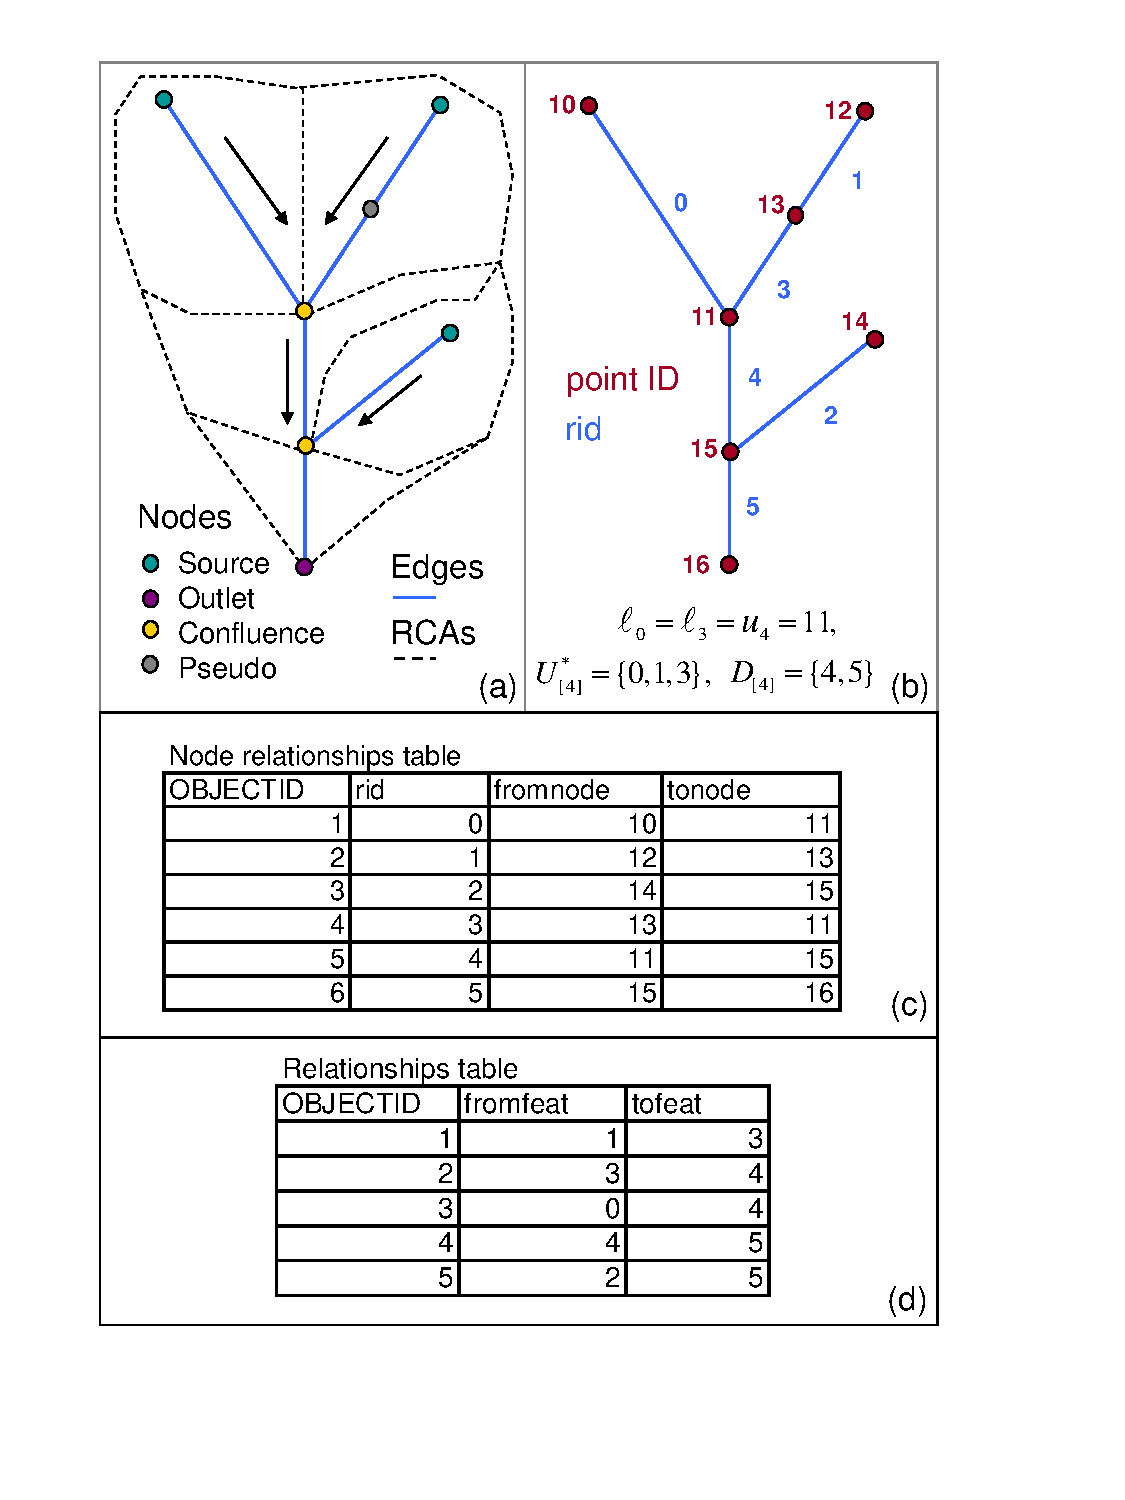
\includegraphics[width=300pt,keepaspectratio]{Figures/Fig1.pdf}
  \end{center}
  \caption{A stream network is made up of a group of directed edges that drain to a single stream outlet (a). Source and outlet nodes occur at the end points of the network, while confluence and pseudo nodes mark locations where edges intersect one another (a). Reach contributing areas (RCAs) form a tessellation of non-overlapping polygons (a). There is a one-to-one relationship between edges and RCAs, which represent the aerial extent that would theoretically contribute overland flow to a given edge. An identifier is allocated to each edge (rid) and node (pointID) in the landscape network (b). The geographic coincidence of nodes and edges is recorded in the noderelationships table (c), while the spatial relationship of edges to one another is stored in the relationships table (d). Both the noderelationships (c) and relationships (d) tables retain information concerning flow direction in the network. \label{Fig1}}
\end{figure}

There are a finite number of stream segments within a network and we
index them arbitrarily using a reach identifier (rid), $j = 1, 2,
\ldots, n$ (Figure~\ref{Fig1}b). Many locations will have the same
upstream distance in a dendritic stream network. Therefore, we denote
each location as $x^j$, which is the upstream distance on the $j$th
stream segment, in order to uniquely define each location and keep
track of upstream distance.  It is also convenient to arbitrarily
assign indices to points in the network, which we denote as $x_i^j$
for the $i$th point, dropping the superscript when knowledge of stream
segment is unnecessary. The most downstream location on the $j$th
segment is denoted as $\ell^j$, and the most upstream location as
$u^j$. As an example, $\ell^0 = \ell^3 = u^4 = x_{11}$
(Figure~\ref{Fig1}b). The whole set of stream segment indices is
denoted as $I$. The index set of stream segments upstream of segment
$j$, including  $j$ is denoted $U_j$, while the index set of stream
segments upstream of segment $j$, excluding  $j$ is denoted as
$U_j^*$. Likewise, the index set of stream segments downstream of
segment $j$, including $j$ is denoted as $D_j$,  while the index set of stream segments downstream of segment $j$, excluding $j$ is denoted as $D_j^*$. As an illustration, $U_4^*=\{0,1,3\}$ and $D_4 = \{4,5\}$ in Figure~\ref{Fig1}b.

% ------------------------------------------------------------------------------
%
%               SECTION THE GIS-BASED SPATIAL MODELING FRAMEWORK
%
% ------------------------------------------------------------------------------

\section{FLoWS geoprocessing toolset}

The ability to quantify and efficiently represent topological
relationships allows users to investigate questions relating to
connectivity, adjacency, proximity, and directional relationships in a
network. However, some common GIS data formats, such as shapefiles and
feature classes, are non-topological data structures; meaning that the
topological relationships between features (e.g., edges) are not
explicitly stored. Instead, topological relationships must be
identified based on the spatial coincidence of features (e.g. edges
intersect at confluences or pseudo nodes (Figure~\ref{Fig1}a), with information
about the nodes, edges, and their topological relationships stored in
attribute and relationship tables \citep{Fish:GIS:2004}. A variety of
topological data models have been developed for use in a GIS; for
example, \code{Vector Networks} are used in \proglang{GRASS} \citep{Nete:Mita:open:2008}, while the \code{Network Dataset} and \code{Geometric Network} are provided in
\proglang{ArcGIS} \citep{ESRI:ArcG:2009}. Often, platform-specific toolsets, such as the
\pkg{v.net} modules for \proglang{GRASS} and the \pkg{Network Analyst} in \proglang{ArcGIS}, are
provided to analyze network data structures. In addition, the \proglang{ArcGIS}
\pkg{Arc Hydro} toolset \citep{Maid:ArcH:2002} is based on the \code{Geometric Network} and
provides an extensive set of tools used to derive new information
about network relationships in streams.

The \pkg{STARS} toolset relies on a \code{LSN}, which is a
topological data model generated using the \pkg{FLoWS} \proglang{ArcGIS} geoprocessing
toolset \citep{Theo:Norm:Pete:Ferr:Wade:func:2006}.  The \pkg{FLoWS} toolset includes a suite of
tools used to analyze relationships in the \code{LSN} data structure, which
have been described elsewhere \citep{Theo:Norm:Pete:Ferr:func:2005,Theo:Norm:Pete:Ferr:Wade:func:2006}. However, we provide an overview of the \code{LSN} structure and a
few particularly useful tools in this section so that users will have
a clear understanding of the underlying data structure that the \pkg{STARS}
toolset depends on; allowing users to generate the same topological
information using other data models and software.

A \code{LSN} is a directional graph used to represent
spatial context and relationships with additional geographic
information \citep{Theo:Norm:Pete:Ferr:Wade:func:2006}. It is created
using the \pkg{FLoWS} toolset and stored as an Environmental Systems
Research Institute (ESRI) \proglang{ArcGIS} personal geodatabase \citep{ESRI:ArcG:2009}. The personal geodatabase is stored as an Access database, which may contain point, polyline (a.k.a. line), and polygon feature classes. Each feature class is made up of similar spatial features and an Access table (i.e., attribute table), which contains attribute data for every spatial feature.

The nodes feature class represents topologic breaks in the stream network such as confluences, stream sources, or stream outlet points, while edges represent flow paths (i.e., line segments) from node to node (Figure~\ref{Fig1}a). The stream reach contributing area (RCA) corresponds to the aerial extent that would theoretically contribute overland flow to a given edge in the absence of other hydrologic processes such as infiltration or evaporation. RCAs have a one-to-one relationship with edges, and form a non-overlapping, contiguous tessellation of polygons (Figure~\ref{Fig1}a). The \pkg{FLoWS} toolset also allows RCAs to be incorporated into the \code{LSN}, but they do not need to be explicitly included for spatial statistical modeling. Instead, landscape characteristics such as land use, elevation, or road density, can be summarized as areas, means, or counts for each RCA, $RCA_j$, and then recorded in the edges attribute table.

The \code{LSN} is based on a ForwardStar data structure \citep{Ahuj:Magn:Orli:netw:1993}, which provides a way to store, search, and calculate new spatial information based on the geographic coincidence of features. These spatial relationships are stored within three tables, which may be related to one another through the node and edge identifiers (\code{pointID} and \code{rid}, respectively). The \code{nodexy} table contains four attributes: the \code{OBJECTID} (internal GIS identifier), \code{pointID}, and the $x$-, $y$-coordinates for each node. The \code{noderelationships} table links the nodes to their associated edges based on the \code{rid}, $j$, and the \code{pointID} (Figures~\ref{Fig1}b,c), while the \code{relationships} table represents the downstream flow paths from edge to edge, which are based on the digitized direction of the line segments. Topological errors are common in GIS data and must be corrected before the \code{LSN} is constructed to ensure that the \code{noderelationships} (Figures~\ref{Fig1}b,c) and \code{relationships} (Figures~\ref{Fig1}b,d) tables accurately represent direction and connectivity within the network. Together, these tables provide a wealth of information about the topology of the network, including the spatial location of each node, the most upstream and downstream location on each edge (\code{fromfeat} = $u^j$ and \code{tofeat} = $\ell^j$, respectively), the direction of the edges, and the spatial relationship between edge features.

One challenge of working with GIS data is that survey sites collected
within a stream usually do not intersect the edge, or segment, where they were collected. This is a common phenomenon that can result for a variety of reasons. Coordinates collected using global positioning system (GPS) units typically have uncertainty associated with them, which translates to locational uncertainty in the site data. Streams have area (i.e., both length and width), but are often represented by lines in a GIS. Consequently, survey sites located on the banks of a stream may not fall directly on a line segment. There are also various degrees of mapping errors and generalizations in digital streams datasets, such as the absence of small tributaries and the homogenization of form. The magnitude of these errors is dependent upon the spatial resolution of the dataset. In addition, the physical location of streams is temporally dynamic, with some segments meandering from their mapped position over time. Regardless of the error source, the survey sites must fall exactly on an edge so that they may be incorporated into the \code{LSN} framework.

The \pkg{FLoWS} tools are used to modify site locations and incorporate site data into the \code{LSN} \citep{Theo:Norm:Pete:Ferr:Wade:func:2006}. This includes both observed site locations where measurements were collected, as well as locations where predictions will be generated. Each site, $s_i$, is associated with an edge using dynamic segmentation. The process involves intersecting the site with the closest edge segment, physically moving the site to the new location, $x_i^j$, and calculating the distance ratio, $r_i$, from the most-downstream location on the edge to the site location:
\begin{equation} \label{eq:ri}
r_i = \frac{d(\ell^j,x_i^j)}{L_j}
\end{equation}
where $d(\ell^j,x_i^j)$ is the distance travelled along edge $j$ (i.e., hydrologic distance) between locations
$\ell^j$ and $x_i^j$ and $L_j$ is the total length of the $j$th edge, $L_j=d(\ell^j,u^j)$.

When the tool has finished successfully, a new point feature class is
created in the \code{LSN} containing the modified site data. The sites
attribute table contains the original attribute data, as well as, a
number of new fields; the most relevant of which are the \code{ratio}
(field type = double), \code{rid} (field type = long), \code{NEAR_X}
and \code{NEAR_Y} (field type = double) fields. The \code{rid} field
indicates which edge the site has been moved to, while \code{ratio}
provides the exact location along the edge. These two pieces of
information allow attributes to be calculated for site-specific
locations. In addition, the \code{NEAR_X} and \code{NEAR_Y} fields
provide the $x$-, $y$-coordinates for the modified site locations,
which are used to calculate the Euclidean distance matrix in the
\pkg{SSN} package.

A \code{LSN} must contain six datasets before it can be used to calculate
the spatial information needed to fit the spatial statistical models
described by \citet{Ver:Pete:Move:2010}: three feature classes
representing the edges, nodes, and survey sites, as well as, three
Access tables containing information about the spatial relationship
between features (Figure~\ref{Fig2}). Additional feature classes
representing prediction locations may also be included. This
information is used to navigate up and downstream between features,
allowing new attributes to be generated based on spatial context and
the relationship between features. As such, the \code{LSN} provides a
powerful and flexible GIS-based hydrologic modeling framework for the
\pkg{STARS} toolset to operate on. For a more detailed description of
the \code{LSN}, please see \citet{Theo:Norm:Pete:Ferr:Wade:func:2006}. For
step-by-step instructions on how to calculate an \code{LSN} appropriate for
spatial statistical modeling in stream networks, please see \citet{Pete:STAR:2011}.
\begin{figure}[htbp]
  \begin{center}
    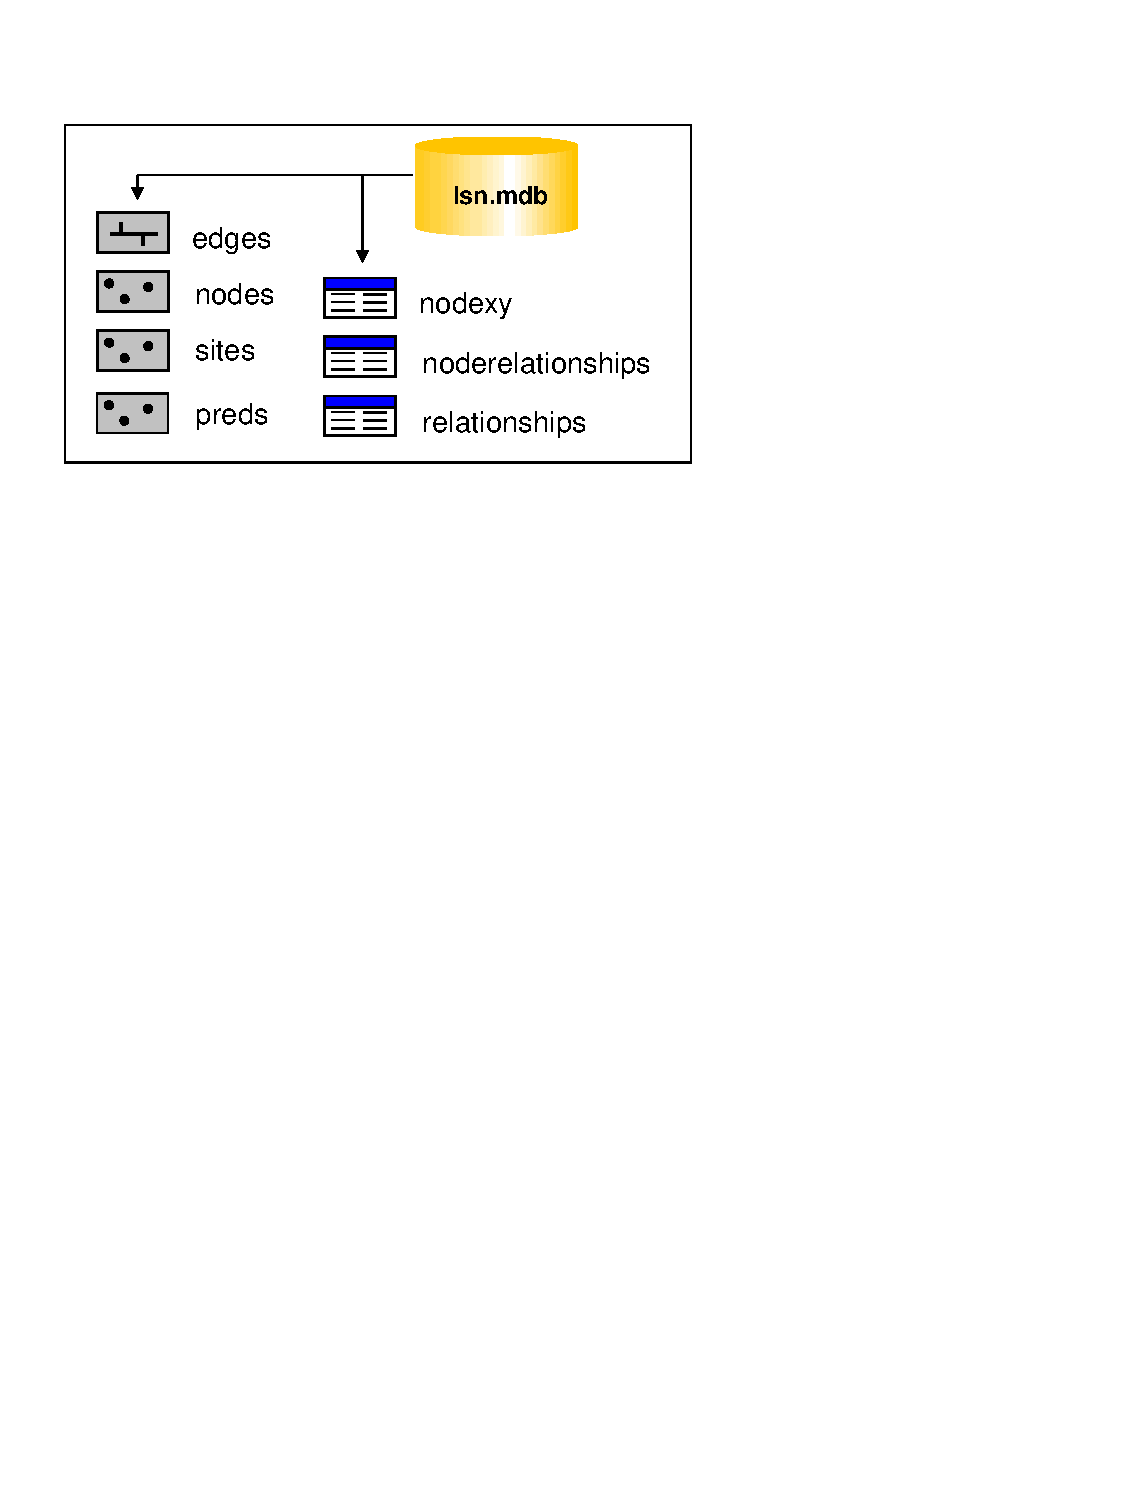
\includegraphics[width=350pt,keepaspectratio]{Figures/Fig2.pdf}
  \end{center}
  \caption{A landscape network (\code{LSN}) must contain six datasets before it can be used to calculate the data needed to fit the spatial statistical models: three feature classes: edges, nodes, and sites, as well as three Access tables: nodexy, noderelationships, and relationships. Additional feature classes representing prediction locations (preds) may also be included. \label{Fig2}}
\end{figure}

% ------------------------------------------------------------------------------
%
%               SECTION STARTS GEOPROCESSING TOOLSET
%
% ------------------------------------------------------------------------------

\section{STARS geoprocessing toolset}

The \pkg{STARS} geoprocessing toolset is used to generate and format
the spatial data needed to fit spatial statistical models to streams
data in the \pkg{SSN} package. These data include information about
hydrologic distances (with flow-direction preserved), the spatial
additive function used to calculate the spatial weights, and the
covariates for all observed and prediction locations in the stream
network. In addition, the topological structure of the network is
exported to a format that can be efficiently stored, accessed, and
analyzed in the \pkg{SSN} package. The \pkg{STARS} toolset was
developed for \proglang{ArcGIS} version 9.3.1
\citep{ESRI:ArcG:2009}, which runs on a \proglang{Windows} operating system,
with scripts written in \proglang{Python} version 2.5
\citep{Hamm:Robi:pyth:2000}.  A \proglang{Python} editor for
\proglang{Windows}, \code{PythonWin} \citep{Hamm:Robi:pyth:2000},
must also be installed to successfully run the toolset.The \pkg{STARS}
toolset contains eight tools that are used to transform an \code{LSN}
into a \code{.ssn} object (Figure~\ref{Fig3}), which is the data
structure the \pkg{SSN} package has been designed to utilize. The
tools are grouped into three general categories: Pre-processing,
Calculate, and Export.

\begin{figure}[htbp]
  \begin{center}
    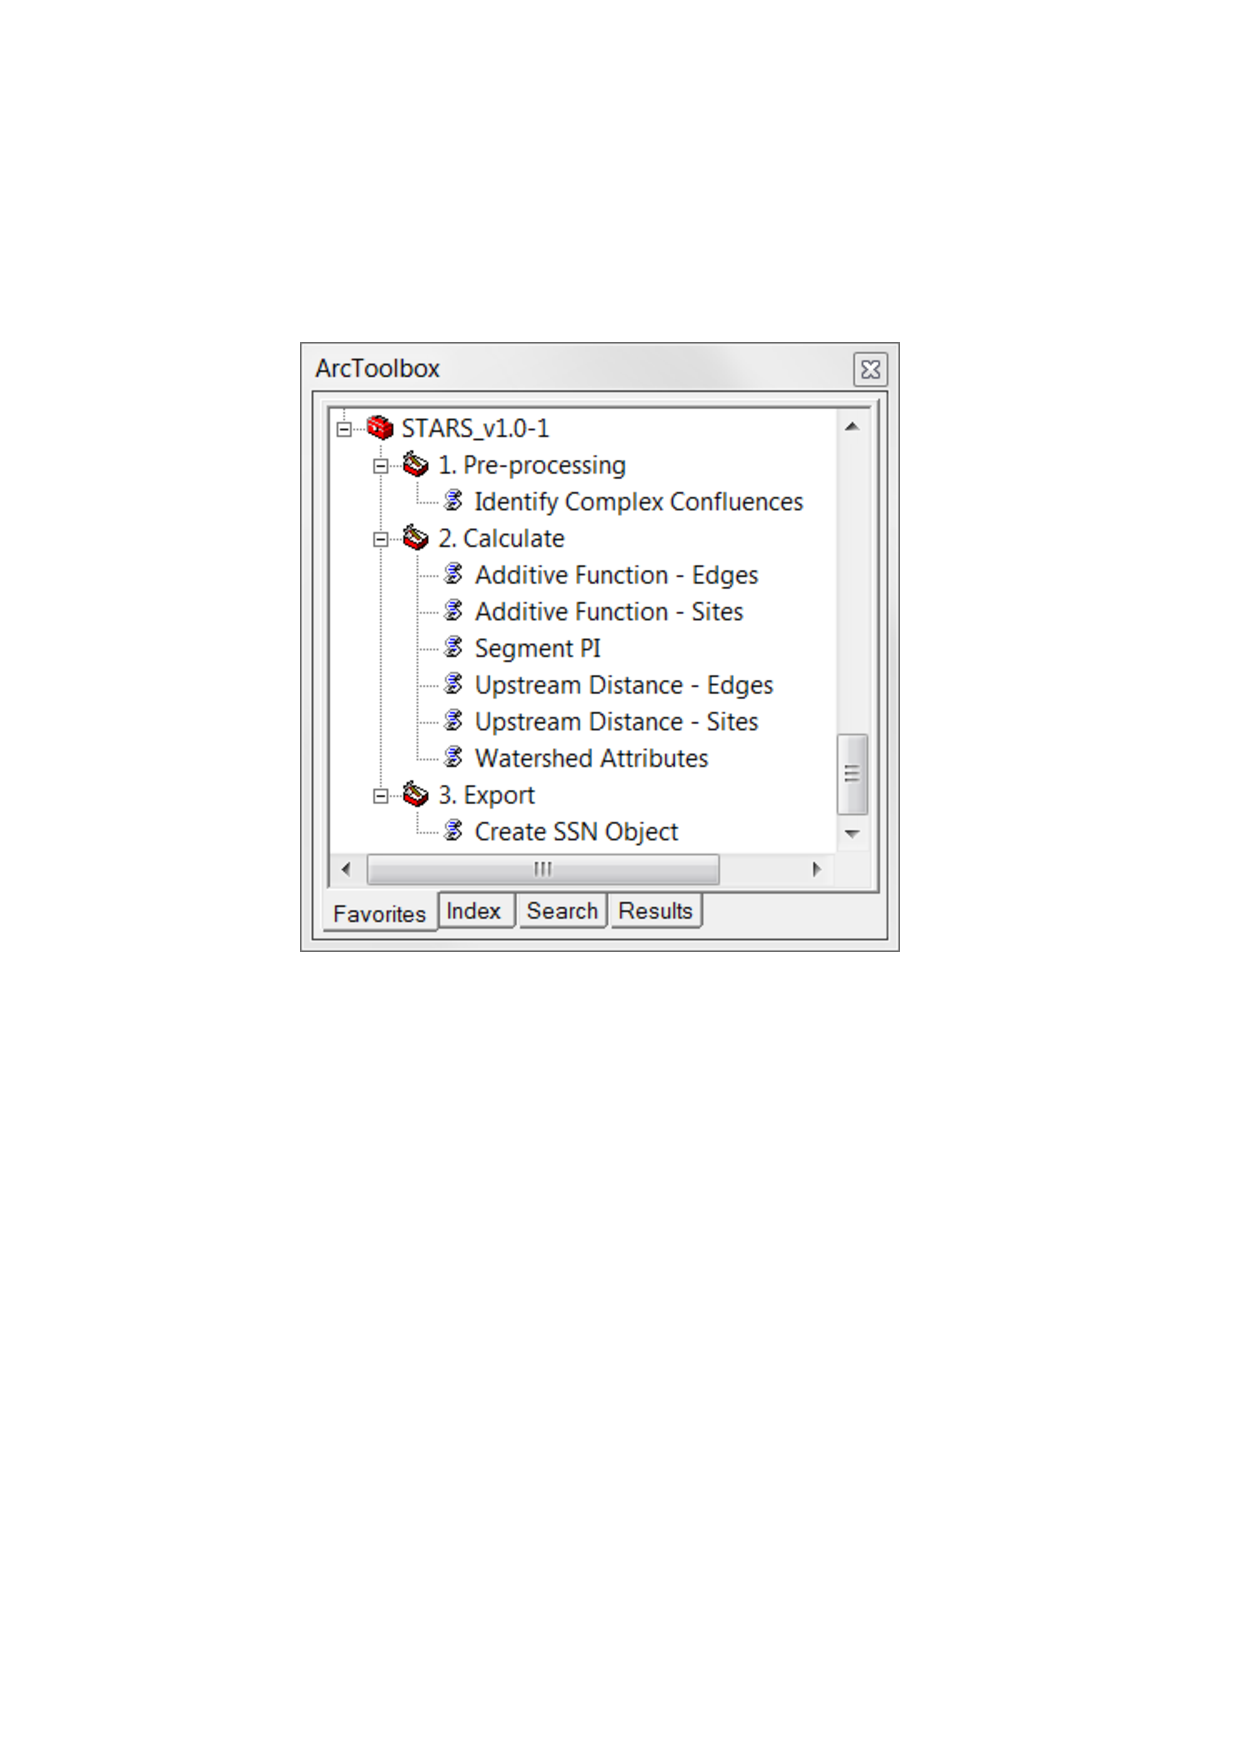
\includegraphics[width=275pt,keepaspectratio]{Figures/Fig3.pdf}
  \end{center}
  \caption{ The \pkg{Spatial Tools for the Analysis of River Systems (STARS)}
toolset contains eight tools that are used to transform a landscape
network into a \code{.ssn} object. The tools are grouped into three general
categories: \code{Pre-processing}, \code{Calculate}, and \code{Export}. \label{Fig3}}
\end{figure}


\subsection{Pre-processing}

\subsubsection{Identify complex confluences}

It is \emph{extremely} critical that the edges are topologically
correct to ensure that hydrologic distances and spatial relationships
are calculated properly using the \pkg{STARS} toolset. The process of
topologically correcting the data can easily be the most
time-consuming aspect of the modeling process, especially for large
datasets. There are a number of useful tools provided in the
\pkg{FLoWS} toolset to help identify and remove errors
\citep{Theo:Norm:Pete:Ferr:Wade:func:2006} and so the majority of the
pre-processing occurs before the final \code{LSN} is generated. However, \code{LSNs}
used to create \code{.ssn} objects have two unique topological
restrictions, which are not considered a true topological error in a
GIS or within a \code{LSN}. First, converging stream nodes are not
allowed. These nodes occur at the downstream node of two edges that
converge (Figures~\ref{Fig4}a,b), but do not flow into another
downstream edge. This commonly occurs at the boundaries of the streams
dataset (Figure~\ref{Fig4}a) or may be the result of topological
errors within the stream network (Figure~\ref{Fig4}b). Converging
nodes are identified using the \pkg{FLoWS} \code{Check Network
  Topology} tool and must be manually removed when the \code{LSN} is being
generated. The second restriction is that only two edges may converge
and flow into a single downstream edge at a confluence. The
\code{Identify Complex Confluences} tool has been included in the
\pkg{STARS} toolset to help users to identify \code{LSN} nodes that violate
this condition (Figure~\ref{Fig4}c). The sole input to the tool is the
\code{LSN} and a text file is produced that contains the \code{pointID} for every node with more than 2
upstream edges (Figure~\ref{Fig5}a). Once these errors have been identified, they must be
manually edited and a new \code{LSN} generated before a \code{.ssn} object
can be created. Note, only the topological relationships shown in
Figure~\ref{Fig1}a are permitted in an \code{LSN} used to generate a spatial
statistical model using the \pkg{SSN} package.
\begin{figure}[htbp]
  \begin{center}
    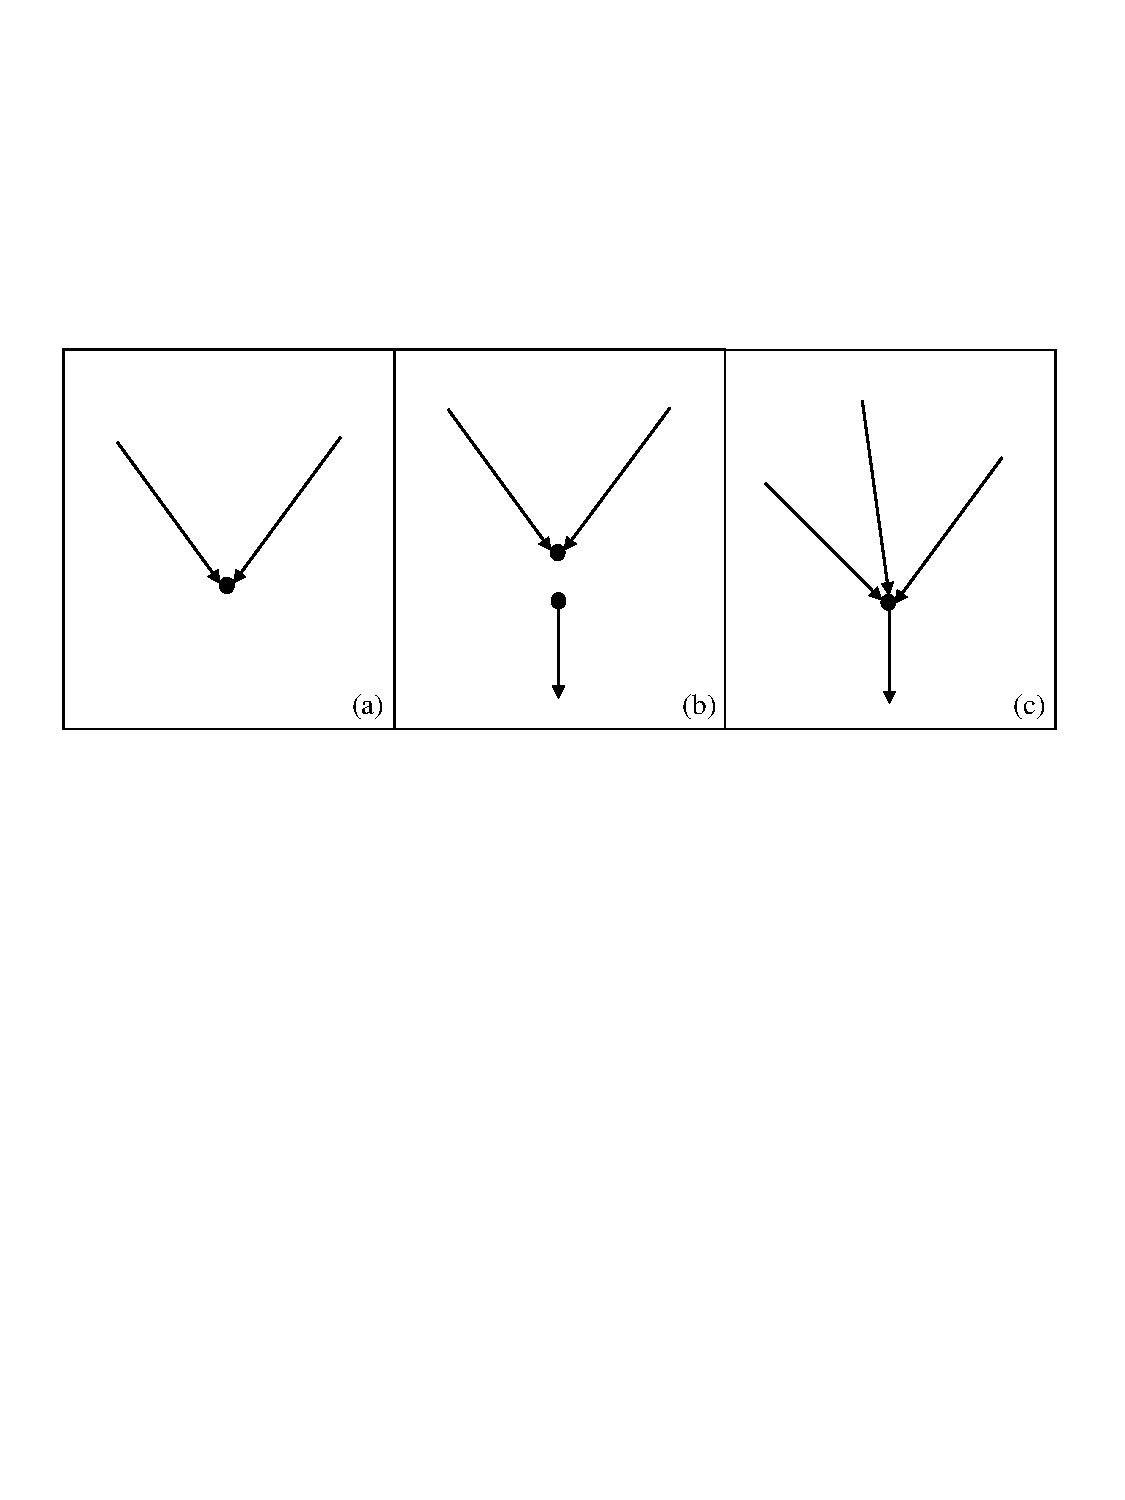
\includegraphics[width=350pt,keepaspectratio]{Figures/Fig4.pdf}
  \end{center}
  \caption{Landscape Networks (\code{LSNs}) used to create \code{.ssn}
    objects have two unique topological restrictions; converging nodes
    (a, b) and complex confluences (c) are not allowed.  Converging
    nodes occur at the downstream node of two edges that converge (a,
    b), but do not flow into another downstream edge. Complex nodes
    occur anytime more than two edges converge at, or flow into, a
    node (c).  \label{Fig4}}
\end{figure}

\begin{figure}[htbp]
  \begin{center}
    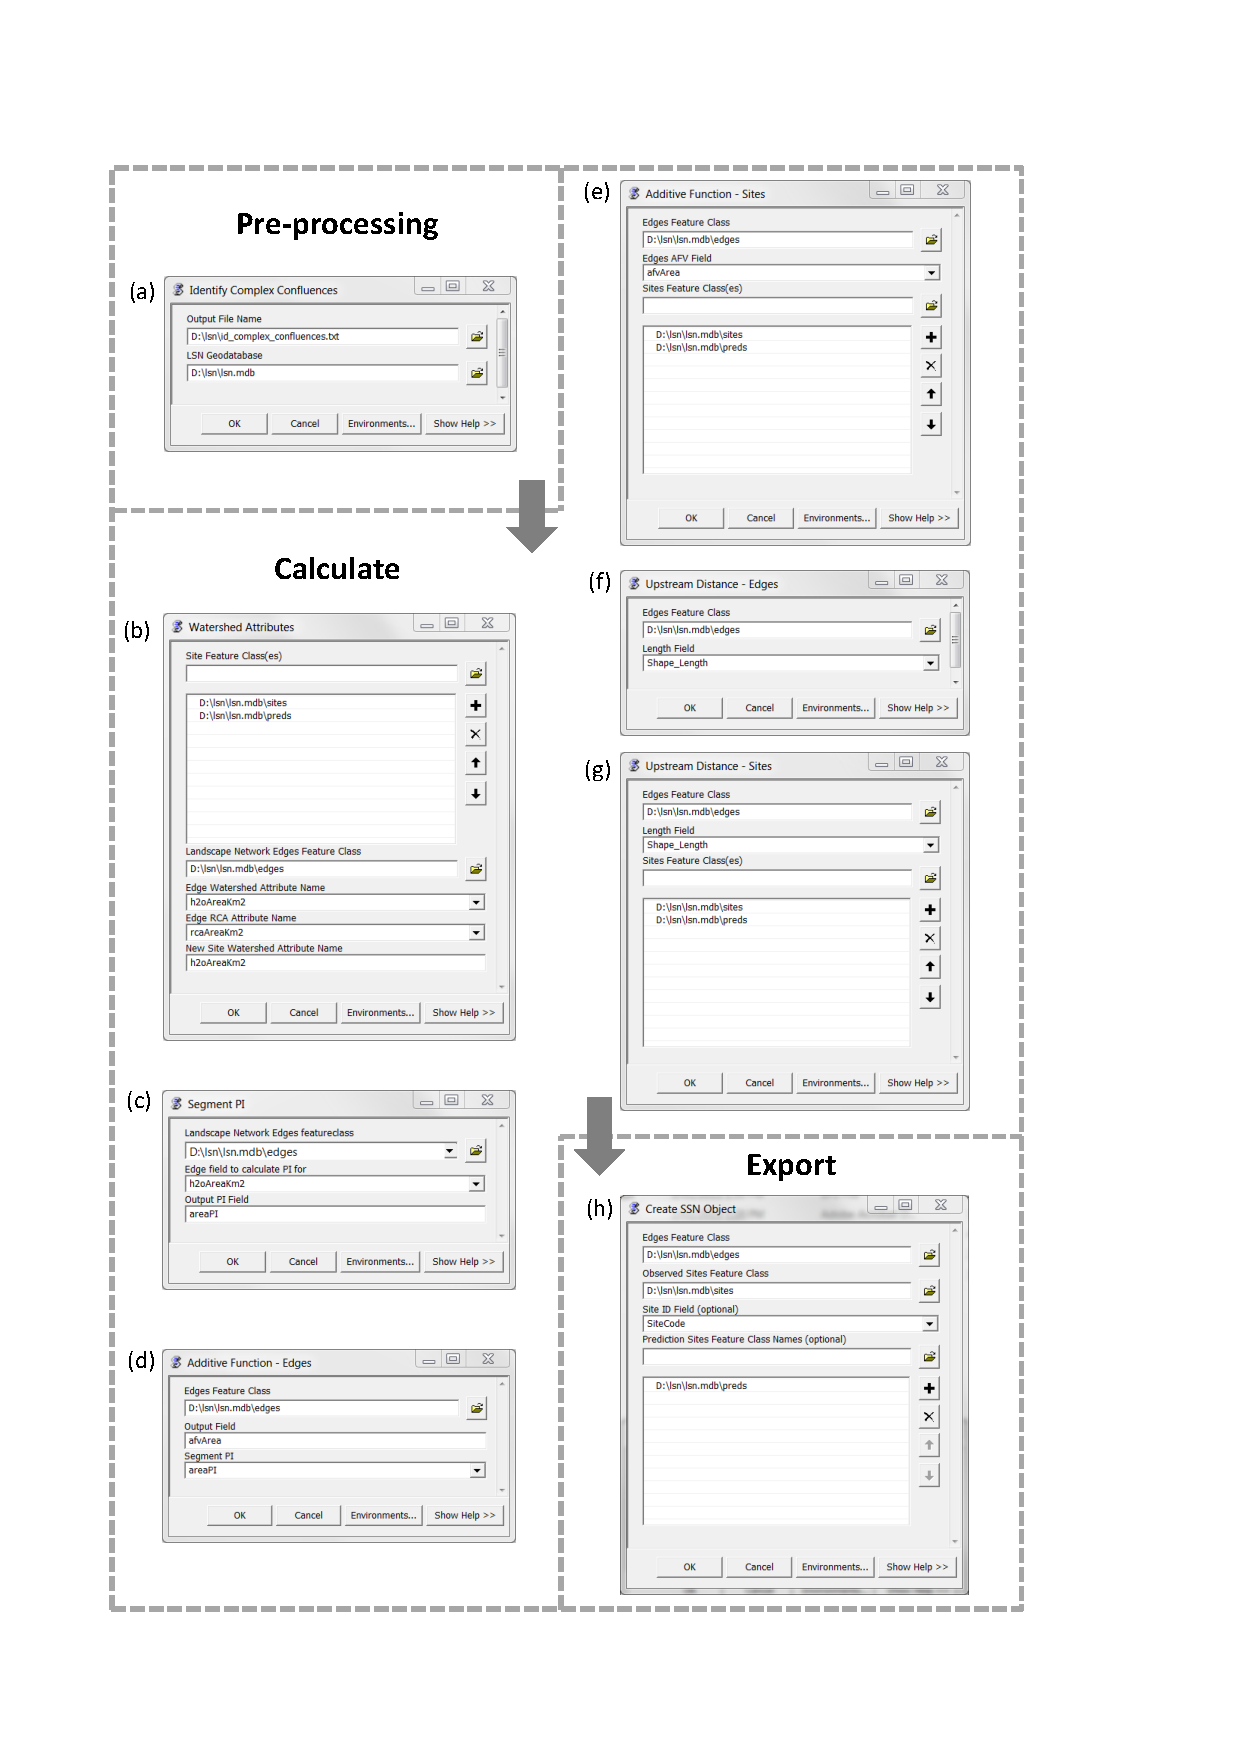
\includegraphics[width=390pt,keepaspectratio]{Figures/Fig5.pdf}
  \end{center}
\caption{Eight tools are included in the \pkg{STARS} geoprocessing toolset: the (a)
\code{Identify Complex Confluences}, (b)\code{Watershed Attributes},
(c) \code{Segment Proportional Influence (PI)}, (d) \code{Additive
Function - Edges}, (e) \code{Additive Function - Sites}, (f) \code{Upstream
Distance - Edges}, (g) \code{Upstream Distance - Sites}, and (h)
\code{Create SSN Object} tools.  \label{Fig5}}
\end{figure}

\subsection{Calculate}

Six tools are provided to calculate the spatial data necessary for spatial statistical modeling: \code{Watershed Attributes}, \code{Segment PI}, \code{Additive Function - Edges}, \code{Additive Function - Sites}, \code{Upstream Distance - Edges}, and \code{Upstream Distance - Sites}.

\subsubsection{Watershed attributes}

The RCA is used to characterize landscape conditions found near each
edge (Figure~\ref{Fig1}a), but in most cases it is only a subcomponent
of the watershed; the exception being source edges where the watershed
and the RCA are equivalent (Figure~\ref{Fig1}a). Instead, the
watershed is commonly used as an analytical unit to summarize
characteristics about the landscape that have the potential to affect
in-stream conditions \citep{John:Host:rece:2010}. For example, common watershed attributes of interest include area, proportional land use or land cover type (e.g. urban area / watershed area), or the number of road crossings upstream. The \pkg{FLoWS} toolset provides the capability to sum edge attributes downstream (\code{Accumulate Values Downstream} tool). When an RCA attribute is summed, a watershed attribute is generated for the most downstream location on each edge. Yet, survey sites may fall anywhere along an edge. The \pkg{STARS} \code{Calculate Watershed Attributes} tool was developed to estimate site-specific watershed attributes:
\[
	W_i=(1-r_i)RCA_i + \sum_{k \in U_i^*}RCA_k
\]
where $W_i$ is the watershed attribute for each survey site $i$,
$RCA_i$ is an attribute summarized over the RCA where the $i$th site
resides, and $r_i$ is as defined in Equation~\ref{eq:ri}. Inputs to
the tool include the sites feature class, the edges feature class, the
watershed attribute name, and the RCA attribute name (Figure~\ref{Fig5}b). A new field
is added to the sites attribute table that contains the $W_i$ for each
site. Note, $W_i$ is simply an estimate of the true watershed
attribute because $RCA_i$ does not contain spatial information about
attribute variability at the sub-RCA level.

Although it is relatively simplistic, the \code{Watershed Attributes}
tool is useful for extracting watershed attributes from publically
available, nationally-attributed stream datasets, such as the United
States NHDPlus \citep{HSC:nati:2007} and
the Australian Hydrological Geospatial Fabric (Geofabric) Surface Network dataset \citep{BOM:aust:2012}. In
both cases, each edge is associated with an RCA; though they are
referred to as catchments and subcatchments in the NHDPlus and
Geofabric, respectively. Environmental attributes, such as land use,
number of road crossings or dams, or climate statistics are provided
at the RCA scale in separate relational databases \citep{Stei:Hutc:Stei:nati:2012, USGS:attr:2010}. These attributes
may be joined to the edges and summed downstream using the \pkg{FLoWS}
\code{Accumulate Values Downstream} tool before extracting estimates of
watershed attributes using the \code{Watershed Attributes}
tool. However, other more spatially-explicit methods may also be used
to calculate site-specific watershed attributes. For example, the
\proglang{ArcGIS} \pkg{Arc Hydro} toolset can be used to calculate
spatially explicit watershed attributes when source data, such as land
use or climate, are available. Raster-based approaches may also be implemented independently
of a topological data model using the
\proglang{ArcGIS} \pkg{Spatial Analyst} extension \citep{ESRI:ArcG:2009},
\pkg{FRAGSTATS} \citep{McGa:Cush:Ene:FRAG:2012}, or a suite of
\proglang{GRASS} toolsets, such as
\pkg{r.stream} \citep{Jasi:Metz:new:2011}, \pkg{r.watershed}, \pkg{r.flow}, and
\pkg{r.stats} \citep{Nete:Mita:open:2008}, among others. In addition, a variety of
deterministic models could also be used to derive watershed
characteristics \citep[e.g.,][]{Rath:Wohl:one:2001}. Given the plethora of
sophisticated and well-documented methods used to extract watershed attributes, automated approaches used to calculate spatially explicit watershed attributes have not been included in the \pkg{STARS} toolset.


\subsubsection{Segment proportional influence}

Calculating the spatial weights needed to fit a spatial statistical model to streams data is a three step process: 1) calculating the segment proportional influence (PI), 2) calculating the additive function values, and 3) calculating the spatial weights \citep{Pete:Ver:mixe:2010}. Steps 1 and 2 are performed using the \pkg{STARS} toolset, while step 3 is undertaken in \proglang{R} using the \pkg{SSN} package.

The PI for each edge, $\omega_j$, is defined as the relative influence
that the $j$th edge, or segment, has on the edge directly
downstream. In the following example, $\omega_j$ is based on watershed
area, but other simple measures, such as Shreve's stream order
\citep{Shre:stat:1966}, could also be used 
\citep[e.g.,][]{Cres:Frey:Harc:Smit:spat:2006}. To begin,
watershed area is calculated for the most downstream location of each
edge in the network: $A^j=\sum_{k \in U_i}RCA_k$, using the
\pkg{FLoWS} \code{Accumulate Values Downstream} tool. When two edges, denoted $j$ and $j^\prime$, join at a node, the PI, $\omega_j$, for the $j$th edge that flows into the node is then:
\[
	\omega_j = \frac{A^j}{A^j + A^{j^\prime}}.
\]
Note that, the $\omega_j$ values for edges directly upstream from a
single confluence always sum to 1 because they are proportions. Inputs
to the \code{Segment PI} tool include the \code{LSN} edges feature
class, as well as, the field in the edges attribute table that will be
used to calculate the segment PI. The tool outputs a new field to the \code{edges}
attribute table (field type = double) that contains $\omega_j$
(Figure~\ref{Fig5}c).


\subsubsection{Additive function - edges and sites}

Two tools have been provided in the \pkg{STARS} toolset, which are used to calculate the additive function value (AFV) for every edge and site in the \code{LSN}: \code{Additive Function - Edges} and \code{Additive Function - Sites}. Separate tools are provided so that the AFV can be calculated for multiple sets of sites without having to recalculate the values for the edges.

The AFV for the $j$th edge, $AFV_j$, is equal to the product of the segment PIs found in the path downstream from the $j$th edge to the stream outlet:
\[
	AFV_j = \prod_{k \in D_j} \omega_k.
\]
Given that $\omega_j$ is a proportion, the $AFV_j$ will always range
between 0 and 1, with the $AFV_j$ for the most downstream edge in the
network equal to 1. The AFV for the $i$th site, $AFV_i$, is simply
equal to the $AFV_j$ of the edge it lies on. As a result, multiple
sites located on a single edge will always have the same AFV
value.

Inputs to the \code{Additive Function - Edges} tool include the
\code{LSN} edges feature class and the segment proportional influence
(PI) value generated using the \code{Segment PI} tool. The \code{LSN}
edges feature class is also an input to the \code{Additive Function -
Sites} tool, as well as, the \code{LSN} sites feature class(es)
that the AFV values will be assigned to. The \code{Additive Function
- Edges} (Figure~\ref{Fig5}d) and \code{Additive Function - Sites}
(Figure~\ref{Fig5}e) tools create a new field in both the edges and
sites attribute tables representing the AFV (field type = double). For
additional details, please see \citet{Pete:Ver:mixe:2010} and \citet{Pete:STAR:2011}.



\subsubsection{Upstream distance - edges and sites}

There are two tools provided in the \pkg{STARS} toolset to calculate
the upstream distance for each of the edges and sites: \code{Upstream
  Distance - Edges} and \code{Upstream
  Distance - Sites}. The \code{Upstream Distance - Edges} tool is used to calculate:
\[
	upDist_j = \sum_{k \in D_j} L_k
\]
where $upDist_j$ is the upstream distance from the stream outlet to the upper end of the $j$th edge ($u^j$) and $L_j$ is the total length of the $j$th edge. The \code{Upstream Distance - Sites} tool is used to compute the upstream distance from the outlet to the $i$th site, $upDist_i$; i.e., the $x$ part of $x_i^j$, and is given by:
\[
	upDist_i = r_i L_i + \sum_{k \in D_j^*} L_k,
\]
where $L_i$ is the total length of the $j$th edge of $x_i^j$ and
recall that $D_j^*$ is the set of all segments downstream of $x_i^j$,
excluding the $j$th segment. 

Inputs to the \code{Upstream Distance - Edges} (Figure~\ref{Fig5}f)
and \code{Upstream Distance - Sites} (Figure~\ref{Fig5}g) tools include the \code{LSN} edges feature class
and the field in the edges feature class that contains the length of
each segment. The sites feature class(es) that the
upstream distance values will be assigned to must also be specified in the
\code{Upstream Distance - Sites} tool. The $upDist_j$ and $upDist_i$ values are
recorded in the edges and sites attribute tables, respectively, within
a new field named \code{upDist} (field type = double). The information
stored in the two upstream distance attributes provides part of the
spatial information needed to calculate pair-wise hydrologic distances
between locations in the \pkg{SSN} package.



\subsection{Export}

\subsubsection{Create SSN object} \label{createLSN}

The purpose of the \code{Create SSN Object} tool  is to reformat the
feature geometry, attribute data, and topological relationships of
each spatial dataset contained in the \code{LSN} into a \code{.ssn} object so that it can be imported into \proglang{R} using functions provided in the \pkg{SSN} package. As we mentioned previously, a new directory is created to store this information, with the naming convention \code{lsn-name.ssn} (i.e., \code{lsn.ssn}); we refer to this as the \code{.ssn} object (Figure~\ref{Fig6}).

\begin{figure}[htbp]
  \begin{center}
    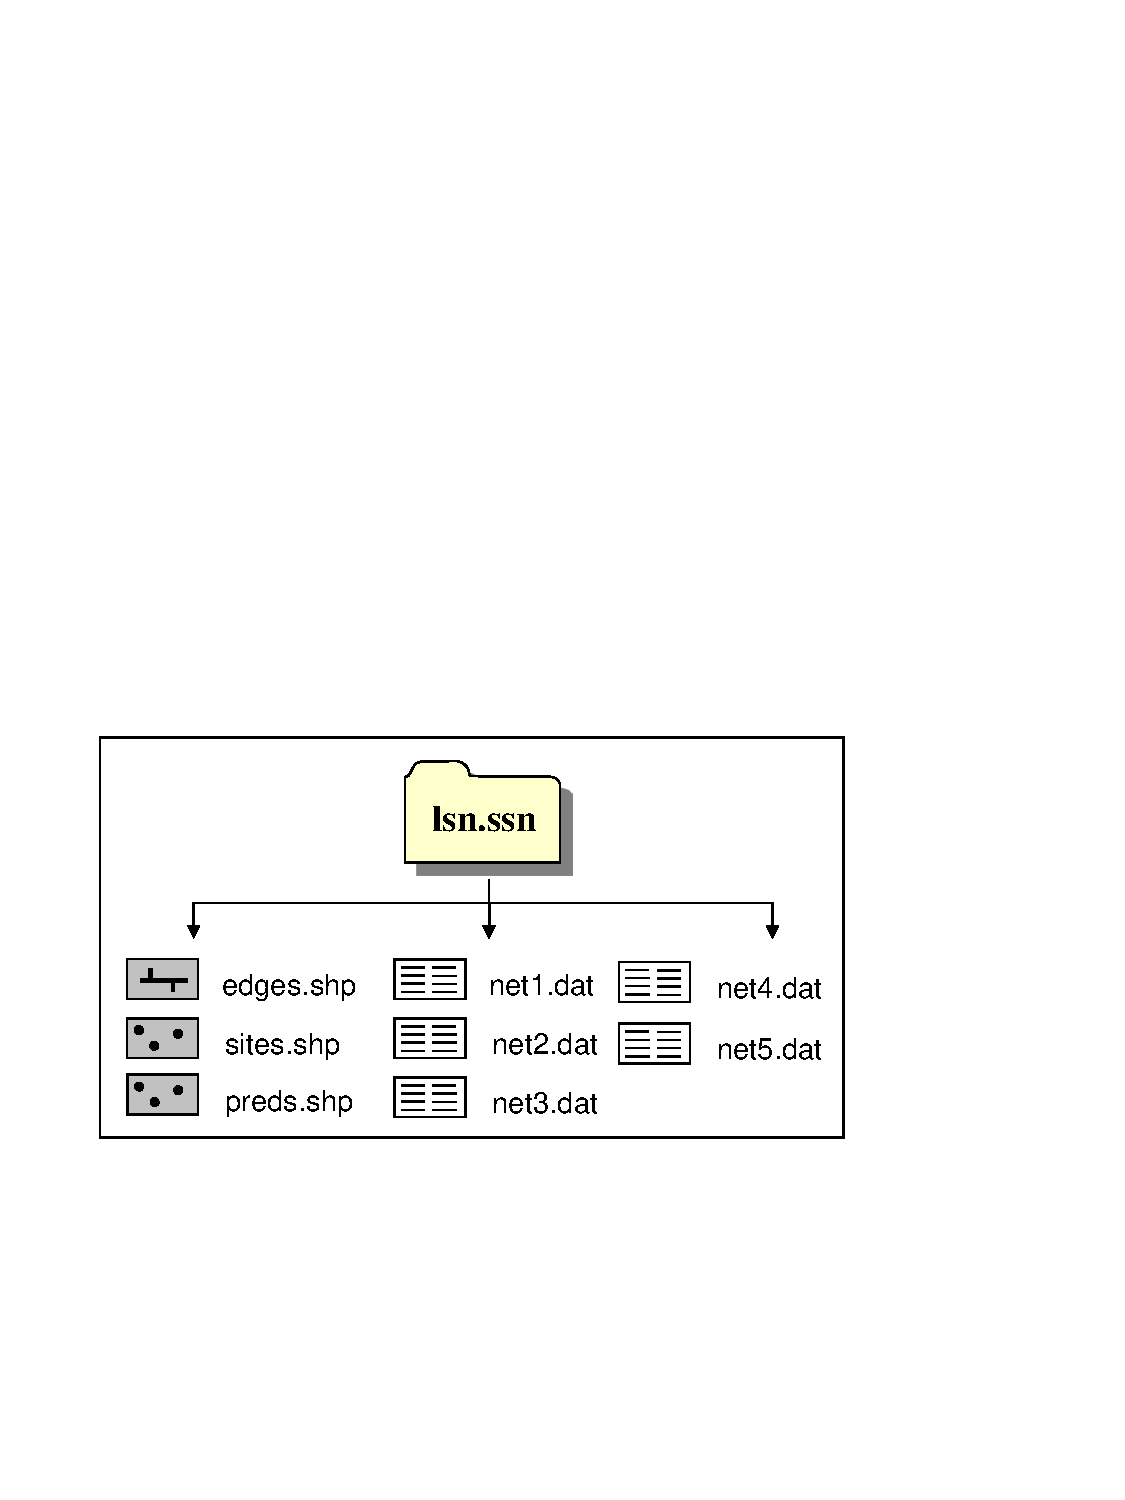
\includegraphics[width=350pt,keepaspectratio]{Figures/Fig6.pdf}
  \end{center}
  \caption{The \code{.ssn} object contains the spatial, attribute, and topological information of the landscape network (\code{LSN}). It will always contain two shapefiles: edges and sites, as well as multiple text files containing the edge binary identifiers for each stream network in the \code{LSN}. Multiple shapefiles representing the prediction locations may also be included.   \label{Fig6}}
\end{figure}

Shapefiles can be easily imported into \proglang{R} using the \pkg{maptools} package \citep{Biva:Pebe:Gome:appl:2008}, with all of the associated shape geometry and attributes. Consequently, the spatial datasets (edges and sites) are converted from \citet{ESRI:ArcG:2009} feature class to shapefile format and stored in the \code{.ssn} object directory. However, shapefiles in standard form cannot be used to represent the topological relationships of the \code{LSN}. Our solution was to generate network and binary identifiers (IDs), which provide an efficient way to assess connectivity and spatial relationships between features on the network.

The process of assigning binary IDs is relatively straightforward. First, the outlet edge (i.e., the most downstream edge in the network) is identified and assigned a binary ID equal to 1 (Figure~\ref{Fig7}). The information stored in the relationships table (Figure~\ref{Fig1}d) is used to identify edges that are directly upstream from the outlet edge. Binary IDs are assigned to the upstream edge(s) by arbitrarily appending a 0 or 1 to the downstream binary ID. For example, binary IDs 10 and 11 are directly upstream from binary ID 1 in Figure~\ref{Fig7}. This process of moving upstream and assigning binary IDs continues until every edge in the stream network has been assigned a binary ID.
\begin{figure}[htbp]
  \begin{center}
    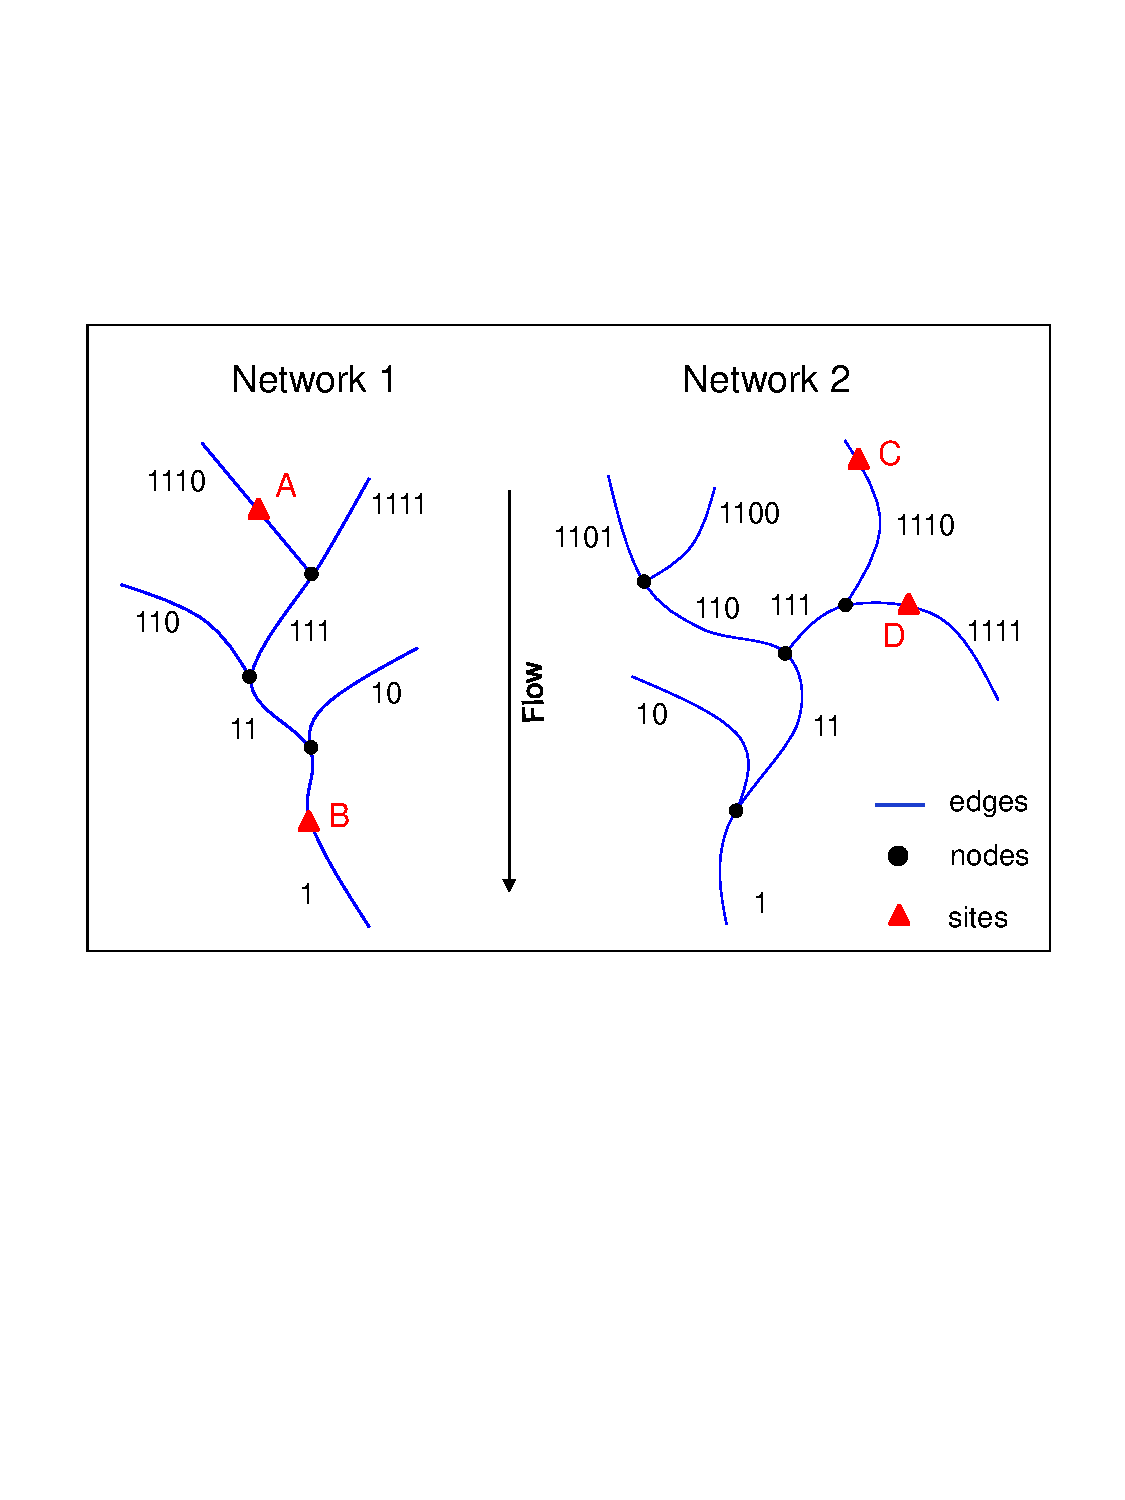
\includegraphics[width=350pt,keepaspectratio]{Figures/Fig7.pdf}
  \end{center}
  \caption{Binary identifiers (\code{binaryID}) are assigned to each edge in the landscape network. \label{Fig7}}
\end{figure}

The binary IDs are useful because they contain information about whether locations have a flow-connected or flow-unconnected relationship. Two locations are considered flow-connected when water flows from an upstream location to a downstream location. In contrast, two locations are flow-unconnected when they share a common outlet downstream, but water does not flow between them. In Figure~\ref{Fig7}, the binary ID for the edge where site B resides is completely nested within the binary ID for the edge where site A lies (``1'' is nested within ``1110''), which indicates that the two locations are flow-connected. In contrast, the binary IDs for the edges where sites C and D reside are not nested (``1110'' is not nested within ``1111'') because the two locations are flow-unconnected. The binary IDs for flow-unconnected locations also contain information about the closest common downstream location. As an example, the most common downstream confluence between sites C and D is $u^{111}$ (Figure~\ref{Fig7}) and so ``111'' is where the two binary IDs diverge.

It is common for \code{LSNs} to contain multiple stream networks, with unique
stream outlets. As an example, consider a streams dataset with two
individual stream networks in the edges feature class
(Figure~\ref{Fig7}). In this case, two edges from different networks
will have the same binary ID. Thus, a network identifier
(\code{netID}, field type = long) is also assigned to the edges,
sites, and prediction sites (if included) attribute tables to differentiate between locations. In addition, a
location ID (\code{locID}, field type = long) and a unique point ID
(\code{pid}, field type = long) are assigned to the sites and
prediction sites attribute tables in order to distinguish between repeated measurements at a single location.

Inputs to the \code{Create SSN Object} tool include the \code{LSN}
edges feature class and the \code{LSN} observed sites feature
class (Figure~\ref{Fig5}h). Optional inputs include a site identifier (ID) field and a
prediction sites feature class. As an output, the \code{Create SSN
  Object} tool stores the \code{rid} and \code{binary ID} for each edge in a
comma delimited text file (Figure~\ref{Fig8}), with a separate file
for each network. The naming convention for these files corresponds to
the network ID (i.e., \code{net1.dat}, \code{net2.dat}, etc.).  Once
the binary and network IDs have been calculated, the edges, sites, and
prediction sites feature classes are converted to shapefiles and
exported to the \code{.ssn} object directory. When the \code{Create
  SSN Object} tool is complete, the \code{.ssn} object will have the file structure shown in Figure~\ref{Fig6} and will contain the information necessary to fit a spatial statistical model using the \pkg{SSN} package.

\begin{figure}[htbp]
  \begin{center}
    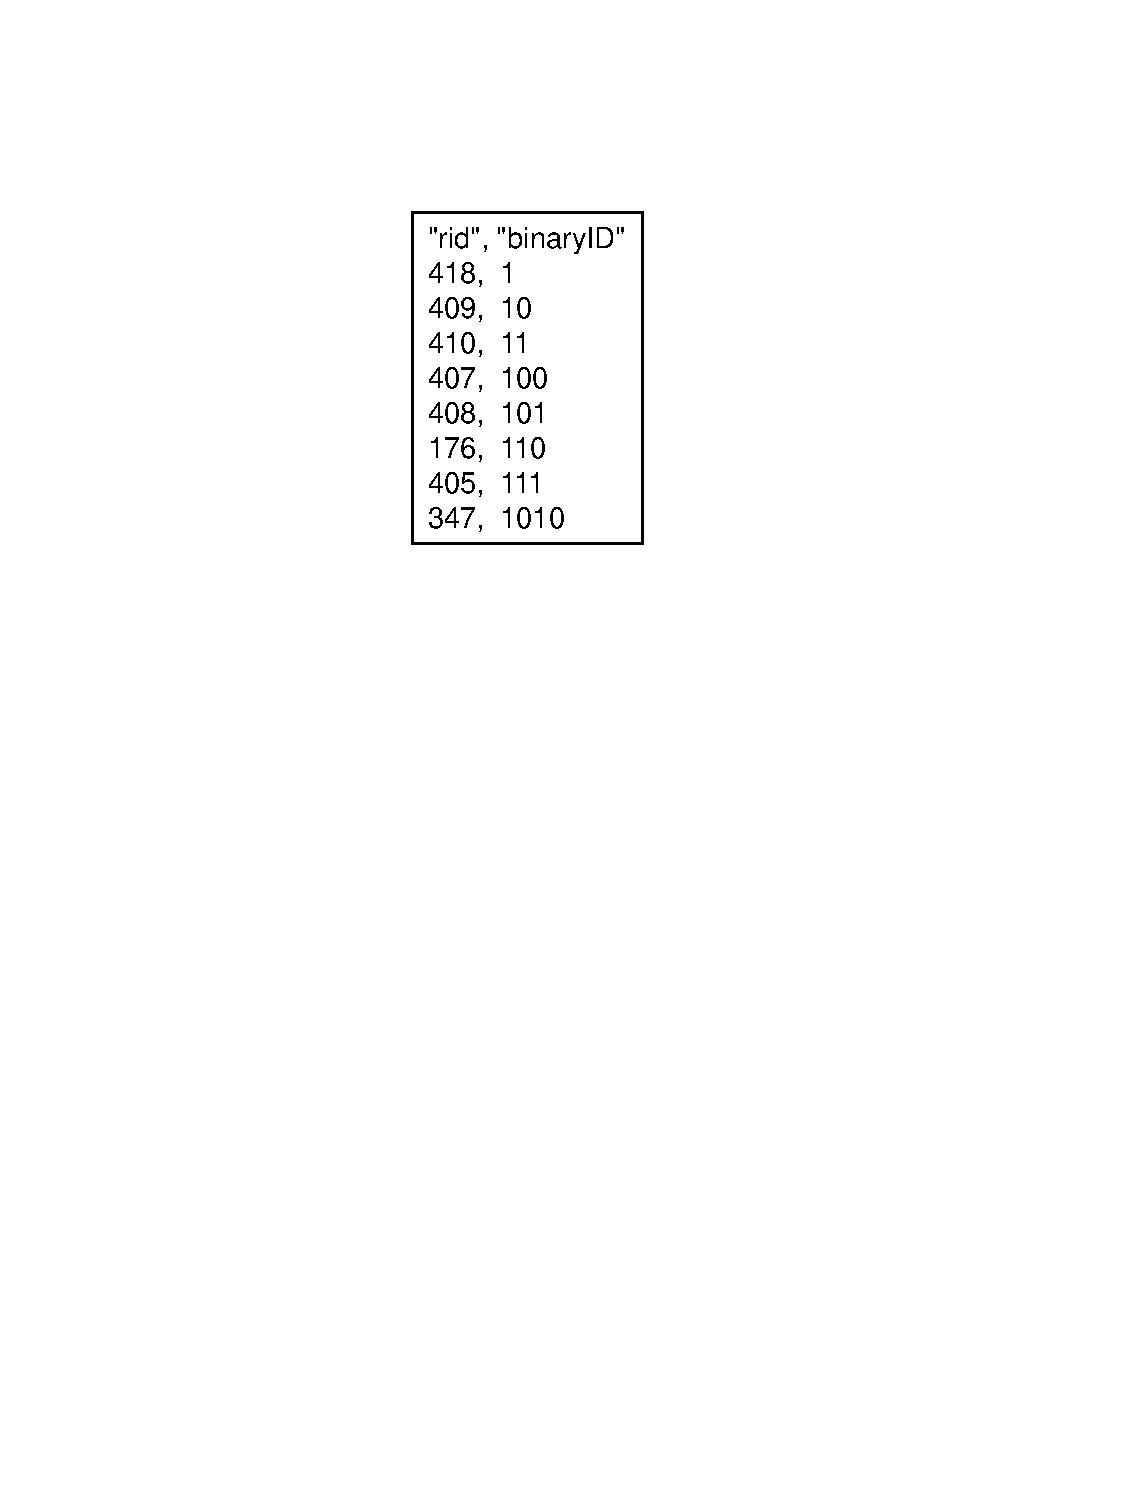
\includegraphics[width=100pt,keepaspectratio]{Figures/Fig8.pdf}
  \end{center}
  \caption{Binary identifiers (IDs) and their associated reach identifier (\code{rid}) are stored in a comma delimited text file format within the \code{.ssn} object. \label{Fig8}}
\end{figure}

% ------------------------------------------------------------------------------
%
%               SECTION ACCESSING THE TOOLS
%
% ------------------------------------------------------------------------------

\section{Accessing the tools}

The \pkg{FLoWS} and \pkg{STARS} custom \proglang{ArcGIS} toolsets, as
well as the \pkg{SSN} package for \proglang{R} statistical software,
are freely available through the ``SSN and STARS'' website hosted by
the U.S. Forest Service, Boise Aquatic Science Lab
\url{http://www.fs.fed.us/rm/boise/AWAE/projects/SpatialStreamNetworks.shtml}. A
tutorial for \pkg{STARS} \citep{Pete:STAR:2011} is also available from the website; it is written for users who have relatively little experience with GIS and provides detailed instructions about how to generate the spatial information needed to fit spatial statistical models for stream networks \citep{Ver:Pete:Move:2010}. An example dataset is available for download and is referred to throughout the tutorial.

% ------------------------------------------------------------------------------
%
%               SECTION FUTURE DEVELOPMENTS
%
% ------------------------------------------------------------------------------

\section{Future developments}

The \pkg{STARS} toolset contains all of the functionality
needed to create the \code{.ssn} object, which can then be imported
into the \pkg{SSN} package and used to fit a spatial statistical model
to stream data.  The \code{LSN} is currently stored as a personal
geodatabase, which provides a self-contained data structure for
multiple feature types (e.g., edges, nodes, survey sites). However,
the personal geodatabase is not a recommended data format in
\proglang{ArcGIS} versions released after 9.3. Therefore, the next
major development will be to select a new data format for the \code{LSN}. The
\proglang{ArcGIS} file geodatabase provides a straight-forward
alternative; it is similar in structure to the personal geodatabase
and an application programming interface (API) has been released for
32 and 64-bit \proglang{Windows} and \proglang{Linux} OS, which should
provide better non-ArcObjects based access to the data. In addition,
the \pkg{FLoWS} and \pkg{STARS} toolsets could be merged to provide a single
custom toolset solely used for spatial statistical modeling on stream
networks. A second alternative is to redesign the \pkg{STARS} tools to take
advantage of the ESRI \code{Geometric Network} and the \pkg{Arc Hydro} toolset. \pkg{Arc
Hydro} does not currently provide out-of-box tools to calculate and
format the spatial information needed to create a \code{.ssn}
object. However, a conversion to this data model would allow users to
take advantage of the extensive set of stream-network analysis tools
provided in \pkg{Arc Hydro}, such as more spatially explicit methods for
calculating, rather than estimating, watershed attributes. A third
alternative would be to recreate the \pkg{FLoWS} and \pkg{STARS}
functionality in an open-source GIS software, such as \proglang{GRASS}
\citep{GRAS:geog:2008}, that can be directly linked with \proglang{R}
using the \pkg{spgrass6} package \citep{Biva:Pebe:Gome:appl:2008}. Although the third alternative
requires more labor to implement, it is attractive for a number of
reasons. First, the ability to link an active GIS session directly
with \proglang{R} reduces the chances of user error when files are
transferred between software packages. Second, a direct linkage would
allow some of the current functionality, such as calculating
covariates for observed and prediction sites, to be more accessible in
\proglang{R}. This would allow users who are unfamiliar with GIS
software to calculate new covariates without having to move between
software programs. Third, \proglang{ArcGIS} is proprietary software,
while \proglang{R} is open-source with a vast community of
contributors and users. Implementing a modeling framework based on
open-source GIS and statistical software would not only be powerful,
but also philosophically appropriate. In the meantime, we have tried
to provide enough detail about the structure of the \code{.ssn} object
so that users can recreate it using other, proprietary and
non-proprietary GIS software packages and data models if necessary.

% ------------------------------------------------------------------------------
%
%               SECTION ACKNOWLEDGMENTS
%
% ------------------------------------------------------------------------------

\section*{Acknowledgments}

Support for this work was provided by the United States (US) Forest
Service, the US Geological Survey, and the Oregon State Office of the
Bureau of Land Management. Some of this work was conducted as part of
the working group entitled ``Spatial Statistical Models for Stream
Networks,'' supported by the National Center for Ecological Analysis
and Synthesis, a Center funded by NSF (Grant \#EF-0553768), the
University of California, Santa Barbara, and the State of
California. This project also received financial support from the
CSIRO Water for a Healthy Country Flagship, and the NOAA's National
Marine Fisheries Service to the Alaska Fisheries Science
Center. We thank Andy Last, Dona Horan, and Jenny Frieden for their assistance in testing the \pkg{STARS} tools and developing the example dataset included in \url{http://www.fs.fed.us/rm/boise/AWAE/projects/SSN_STARS/software_data.html#doc}. We also thank David Clifford for his constructive review of a previous version of this manuscript. Reference to trade names, and the findings and conclusions in the paper, are those of the authors, and do not imply endorsement by the National Marine Fisheries Service, NOAA.


\bibliography{/media/Hitachi2GB/00NMML/BibTexMaster/bibtex/bib/base/StatBibTex}

\end{document}
